\documentclass[10pt,a4paper]{article}
\usepackage[utf8]{inputenc}
\usepackage{amsmath}
\newcommand{\RomanNumeralCaps}[1]
    {\MakeUppercase{\romannumeral #1}}
\usepackage{amsfonts}
\usepackage{amssymb}
\usepackage{float}
\usepackage{verbatim}
\usepackage{listings}
\usepackage{hyperref}

\usepackage{color} %red, green, blue, yellow, cyan, magenta, black, white
\definecolor{mygreen}{RGB}{28,172,0} % color values Red, Green, Blue
\definecolor{mylilas}{RGB}{170,55,241}
\usepackage{amsmath}
\usepackage{graphicx}
\graphicspath{{C:/Users/adria/Pictures/FYS3150/}} 
\author{Adrian Martinsen Kleven, Simon Schrader}
\title{Project 2}

\lstset{
 	language =C++,   
    frame=tb, % draw a frame at the top and bottom of the code block
    tabsize=4, % tab space width
    showstringspaces=false, % don't mark spaces in strings
    numbers=left, % display line numbers on the left
    commentstyle=\color{green}, % comment color
    keywordstyle=\color{blue}, % keyword color
    stringstyle=\color{red} % string color
}

\begin{document}

\part*{-Project 2 - FYS3150/FYS4150-
}
{\large By Simon Schrader (4150), Adrian Kleven (3150) - autumn 2019
}
\tableofcontents

\listoffigures
\listoftables

 
\clearpage
 
\section{Abstract}

\section{Introduction}
\subsection{Purpose} 
The purpose of this report is to examine the efficacy of certain numerical algorithms in solving simple quantum mechanical systems bound by 3- dimensional harmonic oscillator potentials. Specifically, discretizing the radial Schroedinger equation into a system of linear equations and restating the problem in terms of an eigenvalue problem.\\In solving this eigenvalue problem, another purpose is to compare the relative efficacy of an eigenvalue solver based on Jacobi's method [1], and the C++ armadillo library function.
\subsection{Approach}
Discretizing the Radial Schroedinger equation yields a set of linear equations that by the use of Dirichelet boundary conditions yield an eigenvalue problem of a tridiagonal Toeplitz- matrix. The relevance of this is that the eigenvalues of such a matrix have analytical solutions, which gives a benchmark by which the algorithms can be tested.\\The algorithms are implemented using C++.
\section{Methods}

\subsection{Jacobi's eigenvalue algorithm}\label{jacobi algo}
This algorithm bases itself on the properties of similarity transformations. Assume a real and symmetric matrix $A$ with $n$ eigenvalues $\lambda_1,\lambda_2,...,\lambda_n$. Then there exists a real orthogonal matrix $S$ such that
\begin{equation}\label{eq:1}
S^TAS=\begin{bmatrix}
\lambda_1 & 0 & \cdots & 0 \\
0 & \lambda_2 & 0 & \vdots \\
\vdots & 0 & \ddots & 0 \\
0 & \cdots & 0 & \lambda_n \\
\end{bmatrix}.
\end{equation}
$S$ It can be shown then, that the $j'th$ column of the matrix $S$ is the eigenvector corresponding to the eigenvalue $\lambda_j$ for $j \in [1,2,...,n]$ see Ref. [3], chapter 8.\\\\A matrix $B$ is similar to $A$ if $B=S^TAS$, where $S$ is an orthogonal matrix. It can be shown that \hyperref[proof of same eigenvalues]{\emph{$B$ shares eigenvalues with $A$}}. Though the eigenvectors are not in general the same unless $S^T$ happens to be the identity matrix, but then this whole affair would be rather pointless.\\\\Using this property of the similarity transformation, successive applications of such a transform:
$$
S_N^TS_{N-1}^T...S_1^TAS_1...S_{N-1}S_N
$$
will retain the eigenvalues of the original matrix $A$. If in addition, the matrices $S$ and $S^T$ had the property that they gradually reduced the non- diagonal matrix elements to zero, then several iterations of this would yield a diagonal matrix with the eigenvalues of A along the diagonal(equation \ref{eq:1}).
\subsection{One electron in a 3- dimensional harmonic oscillator potential}
Assuming a centrally symmetric harmonic oscillator potential $V(r) = (1/2)m\omega^2r^2$ and a single electron with orbital angular moment equal to zero, the radial Schroedinger equation reads
\begin{equation*}
-\frac{\hbar^2}{2 m} \frac{1}{r^2} \frac{d}{dr} r^2\frac{d}{dr}R(r)+ V(r) R(r) = E R(r). \hspace{1cm} ref.[3]
\end{equation*}
From here on the equation is scaled in order to express the results in terms of dimensionless variables.\\
substituting $R(r) = (1/r) u(r)$. This simplifies the expression considerably to

\begin{equation*}
  -\frac{\hbar^2}{2 m} \frac{d^2}{dr^2}u(r)+ V(r) u(r) = E u(r).
\end{equation*}
Imposing Dirichelet boundary conditions, due to the nature of the normalizable wave functions that represent physical systems $u(0)=u(\infty)=0$. Dividing $r$ by the constant $\alpha$ where $[\alpha] = length$ to introduce the dimensionless variable $\rho =\frac{r}{\alpha}$, $V(\rho)$ becomes $\frac{1}{2}k\alpha^2 \rho^2$. The equation becomes

\begin{equation*}
  -\frac{\hbar^2}{2 m \alpha^2} \frac{d^2}{d\rho^2} u(\rho) 
       + \frac{k}{2} \alpha^2\rho^2u(\rho)  = E u(\rho) .
\end{equation*}
To get a factor of 1 in front the second derivative term, both sides of the equation are multiplied by $2m\alpha^2/\hbar^2$

\begin{equation*}
  -\frac{d^2}{d\rho^2} u(\rho) 
       + \frac{mk}{\hbar^2} \alpha^4\rho^2u(\rho)  = \frac{2m\alpha^2}{\hbar^2}E u(\rho) .
\end{equation*}
Then the value of $\alpha$ is fixed so that the factor in front of the second term on the LHS is 1

\begin{equation*}
\alpha = \left(\frac{\hbar^2}{mk}\right)^{1/4}.
\end{equation*}
Defining

\begin{equation*}
\lambda = \frac{2m\alpha^2}{\hbar^2}E,
\end{equation*}
Schroedinger's equation is then written as

\begin{equation*}
  -\frac{d^2}{d\rho^2} u(\rho) + \rho^2u(\rho)  = \lambda u(\rho) .
\end{equation*}
In order to discretize this, the expression for the second derivative

\begin{equation*}
  \frac{u(\rho+\epsilon) -2u(\rho) +u(\rho-\epsilon)}{\epsilon^2}
\end{equation*}
is used.\\As infinity cannot be represented in a computer, a maximal value $\rho_{max}$ is used, at which the wave function approaches zero within a predetermined tolerance. Then, choosing a number of mesh points N from which the step length $h=\frac{\rho_N-\rho_0 }{N+1}$ is decided, $\rho$ can be discretized as $\rho_i= \rho_0 + ih$ where $i=1,2,\dots , N$ and $u(\rho_i)=u_i$. The following expression is then arrived at for the Schroedinger equation for a given $\rho_i$:

\begin{equation*}
-\frac{u_{i+1} -2u_i +u_{i-1}}{h^2}+\rho_i^2u_i= \lambda u_i
\end{equation*}
From here the matrix elements are defined from the coefficients of $u_{i+1}$, $u_{i}$, and $u_{i-1}$ .$u_0 = u(0)= 0$ and $u_N = u(\rho_{max}) \approx 0$ and so are exempt from the matrix, giving a $N-1 \times N-1$ matrix and corresponding eigenvalue problem:
$$
d_i=\frac{2}{h^2}+\rho_i^2,\hspace{1cm}  a=-\frac{1}{h^2}
$$
\begin{equation*}
\begin{bmatrix}
d_1 & a &0  &0  &\cdots  & 0\\ 
 a&  d_2& a & 0 & \cdots &0 \\ 
 0&  a&  d_3& \ddots  &\ddots  &\vdots \\ 
 0& 0 & a &  \ddots& a &0 \\ 
 \vdots&\vdots  &\ddots  &\ddots  &  d_{N-2}&a \\ 
 0& 0 & \cdots & 0 & a &d_{N-1}& 
\end{bmatrix}
  \begin{bmatrix} u_{1} \\
                                                              u_{2} \\
                                                              \vdots\\ \vdots\\ \vdots\\
                                                              u_{N-1}
             \end{bmatrix}=\lambda \begin{bmatrix} u_{1} \\
                                                              u_{2} \\
                                                              \vdots\\ \vdots\\ \vdots\\
                                                              u_{N-1}
             \end{bmatrix}.  
      \label{eq:sematrix}
\end{equation*}
From here, a number of algorithms can be used in fishing out the eigenvalues and corresponding eigenvectors. \hyperref[jacobi algo]{\emph{The Jacobi eigenvalue algorithm}} can be applied to any real, symmetric matrix, and so it will be applied here.
\subsection{Two electrons in a 3- dimensional harmonic oscillator potential}



\subsection{C++ Implementation}
\subsubsection{One electron in a 3- dimensional harmonic oscillator potential}

\subsubsection{Two electrons in a 3- dimensional harmonic oscillator potential}

\subsubsection{...}

\subsection{Accuracy}

\section{Results}


\begin{figure}[H]
	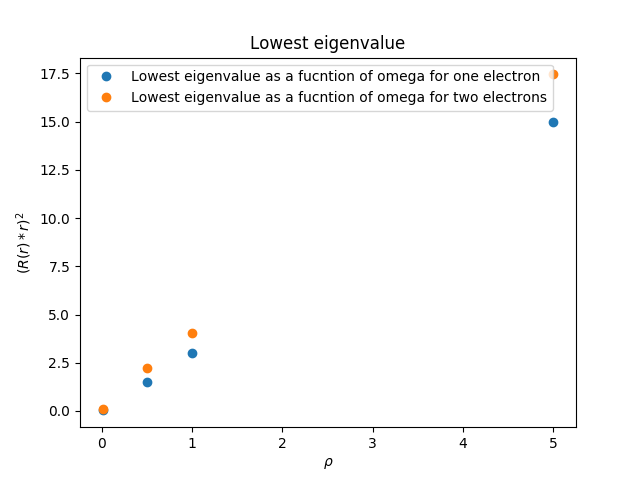
\includegraphics[width =1.2\textwidth]{eigenvalues.png}
	\caption[Lowest eigenvalues of the single- and double- electron systems as a function of $\omega$]{figure text}
\end{figure}

\begin{figure}[H]
	\includegraphics[width =1.2\textwidth]{ground_state_comparision_omega_1_000000.png}
	\caption[Ground states of the single- and double- electron systems]{Ground states of the single- and double- electron systems compared under $\omega =1.000$}
\end{figure}

\begin{figure}[H]
	\includegraphics[width =1.2\textwidth]{solutions_one_electron_0_010000.png}
	\caption[contents title]{figure text}
\end{figure}

\begin{figure}[H]
	\includegraphics[width =1.2\textwidth]{solutions_one_electron_0_500000.png}
	\caption[contents title]{figure text}
\end{figure}

\begin{figure}[H]
	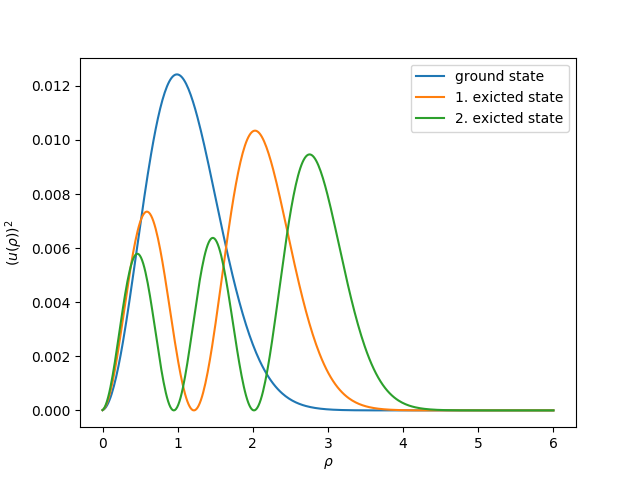
\includegraphics[width =1.2\textwidth]{solutions_one_electron_1_000000.png}
	\caption[contents title]{figure text}
\end{figure}

\begin{figure}[H]
	\includegraphics[width =1.2\textwidth]{solutions_one_electron_5_000000.png}
	\caption[contents title]{figure text}
\end{figure}

\begin{figure}[H]
	\includegraphics[width =1.2\textwidth]{solutions_two_electrons_0_010000.png}
	\caption[contents title]{figure text}
\end{figure}

\begin{figure}[H]
	\includegraphics[width =1.2\textwidth]{solutions_two_electrons_0_500000.png}
	\caption[contents title]{figure text}
\end{figure}

\begin{figure}[H]
	\includegraphics[width =1.2\textwidth]{solutions_two_electrons_1_000000.png}
	\caption[contents title]{figure text}
\end{figure}

\begin{figure}[H]
	\includegraphics[width =1.2\textwidth]{solutions_two_electrons_5_000000.png}
	\caption[contents title]{figure text}
\end{figure}


\subsection{Precision}

\subsection{Time expenditure}

\section{Conclusion}

\section{Critique}

\section{Appendix}
\subsection{Proof that similar matrices share eigenvalues}\label{proof of same eigenvalues}
If a matrix $B$ is similar to a matrix $A$, then $B=S^{-1}A^S$. Then if $\vec{x}$ is an eigenvector of $A$ with eigenvalue $\lambda$:
$$
A\vec{x}=\lambda\vec{x}
$$
Both sides of the equation can be multiplied by $S^{-1}$ and the identity operator $I = SS^{-1}$ can be inserted in between $A$ and $\vec{x}$ to yield
$$
S^{-1}ASS^{-1}\vec{x} =B\left(S^{-1}\vec{x}\right)= \lambda \left( S^{-1}\vec{x}\right)
$$
So $\lambda$ is also an eigenvalue of $B$ though with the corresponding eigenvector $\left( S^{-1}\vec{x}\right)$.
\subsection{List of programs}
All programs can be found on \url{https://github.com/adrian2208/FYS3150_collab}
\begin{enumerate}
\item 
\end{enumerate}
\subsection{Tables}


\section{References}
\begin{itemize}
\item[(1)] Jacobi, C.G.J. (1846). "Über ein leichtes Verfahren, die in der Theorie der Säkularstörungen vorkommenden Gleichungen numerisch aufzulösen". Crelle's Journal (German)
\item[(2)] Morten Hjort-Jensen \textit{Computational Physics: Lecture Notes Fall 2015}
\item[(3)]G. Golub, C. Van Loan, Matrix Computations (John Hopkins University Press, 1996)
\end{itemize}


\begin{comment}

$$
\begin{bmatrix}
0 & 0 & 0 & 0 \\
0 & 0 & 0 & 0 \\
0 & 0 & 0 & 0 \\
0 & 0 & 0 & 0 \\
\end{bmatrix}
$$

\begin{lstlisting}[caption=insert caption]
for (unsigned int i = 0; i<100;i++{
}
\end{lstlisting}

\begin{figure}[h]
\includegraphics[width=8cm]{}
\caption{include caption}
\end{figure}

\end{comment}

\end{document}